\documentclass[12pt]{article}
\usepackage{graphicx,amssymb,amsmath,setspace,comment,verbatim,titling,pgf,lscape,color}
\usepackage[left=2cm,right=2cm,top=2.5cm,bottom=2cm]{geometry}
\usepackage[round]{natbib}
\usepackage{hyperref}
\usepackage{array}
\usepackage{bbm}
\usepackage{marginnote}
\usepackage[justification=centering]{caption}
%%\usepackage{breqn}
\newcommand{\pderiv}[2]{\frac{\partial#1}{\partial#2}}
%\usepackage{siunitx}
\newcolumntype{P}[1]{>{\raggedright\arraybackslash}p{#1}}
\hypersetup{colorlinks,%
						citecolor=black,%
						filecolor=black,%
						linkcolor=black,%
						urlcolor=blue,%
						}
\setstretch{1.5}

\setlength{\droptitle}{-50pt}

\begin{document}
\title{Decision Assistance and Steering in Health Insurance}
\author{Ian McCarthy \& Evan Saltzman}
\date{May 2021}
\maketitle

\vspace{-2ex}
\begin{abstract}
\noindent 
\end{abstract}

\clearpage

\section{Introduction}
\label{sec:introduction}

Health insurance markets are unique in many respects, not least of which is the increasing complexity of choosing an optimal health insurance plan. Such complexity has been well-documented in studies of health insurance choice in the Medicare Advantage market \citep{abaluck2011, ketcham2012, gruber2017}. One way to reduce the burden of this complexity is to provide professional decision support through private insurance agents or public assistance programs, both of which are available in the California health insurance exchanges created under the Affordable Care Act (ACA). Such decision assistance, however, also introduces the potential for private insurers to steer enrollees into potentially suboptimal plans. Commissions paid to facilitate any steering may also increase plan premiums for all enrollees. In this paper, we examine the role of decision assistance on health insurance plan choice and its implications for consumer welfare.

Our analysis is based on household enrollment data from the California ACA exchange. Our final data consist of over 3.2 million household-year observations from 2014 to 2019. The data include a variety of household characteristics, plan choices and plan characteristics, and information on the type of decision assistance used by the enrollee (if any). Using these data, we can precisely identify each household's choice set, the premium paid for each plan in the choice set, and any premium and cost sharing subsidies for which the household is eligible.

Our empirical analysis proceeds as follows. First, we examine whether decision assistance affects plan choice. Our estimand of interest is the average treatment effect on the treated (ATT) for enrollees receiving decision assistance. We employ as our estimator an augmented inverse propensity weighted nested logit regression, as discussed in more detail in Section \ref{sec:causal}, and we limit the analysis to newly enrolled households. We estimate that such households are 50\% more likely to select a silver plan and 20\% less likely to remain uninsured when using some form of decision assistance. We also find strong evidence of heterogeneous effects depending on the type of assistance used, wherein households using public decision assistance ...

Second, we consider the potential for decision assistance to ``improve'' plan choice. While identifying ``improvement'' is not generally feasible in our data, we can identify specific instances in which the observed plan choice is dominated by some other plan in an individual's choice set. For example, Gold and Platinum tier plans are dominated for any household that is eligible for cost-sharing subsidies and with incomes below 150\% of the federal poverty level. We can therefore identify dominated choices and examine whether those with decision assistance appear less likely to select a dominated plan. As with our initial nested logit model of plan choice, our estimand is the ATT for households receiving decision assistance, and our estimator is an augmented inverse propensity weighted logit regression. 

Regarding dominated choices, our results suggest that individuals with decision assistance are over 1 percentage point less likely to make a dominated choice. On a base of 3.5\%, this reflects a 30\% decrease in the probability of making a dominated choice. We again find evidence of heterogeneities in the effects of different forms of decision assistance. In particular, we find that individuals using publicly provided decision assistance are around 0.76 percentage points less likely to select a dominated plan, while individuals using a private insurance agent are 1.2 percentage points less likely to select a dominated plan.

Third, 

We contribute to two distinct literatures. First, our examination of decision assistance and health insurance relates to the literature on the role of experts in decision making.

A related literature considers the effects of recommendations, sometimes automated via an algorithmic recommendation, on decisions. \cite{bundorf2019}, for example, show that offering additional information alongside an algorithmic expert recommendation significantly affects an individual's choice of prescription drug plans.

Second, we contribute to the literature examining the prevalence and underlying mechanisms of poor decision making in health insurance. In the employer-provided insurance market, \cite{liu2021} documents that over half of employers offer a dominated plan among their menu of insurance options available to their employees, and \cite{sinaiko2011} and \cite{bhargava2017} find that a large share of employees regularly select such dominated insurance plans. \cite{abaluck2011}, \cite{ketcham2012}, \cite{zhou2012}, \cite{heiss2013}, \cite{gruber2017}, \cite{ho2017rand} and many others similarly examine poor decisions when selecting a Medicare prescription drug (Part D) plan. The consensus from this literature is that individuals regularly make \textit{ex ante} very bad health insurance decisions, often selecting plans that are either financially dominated by other plan options or most likely suboptimal given the enrollee's existing medical conditions.

Specifically in the context of the ACA, \cite{orzol2018} find that an ``Enroll America,'' a national non-profit organization designed to expand health insurance enrollment in the U.S., significantly increased enrollment in the ACA exchange plans. \cite{myerson2019} also finds that federally funded assistance programs significantly increased the probability of enrollment in Medicaid, although they found little effect of such federal funding on enrollment in exchange plans. \cite{sommers2015} similarly show that access to navigators is highly correlated with Medicaid enrollment, mirroring earlier findings from \cite{aizer2003} in her study of Medicaid enrollment and application assistants in California.

\cite{aizawa2021}

While not definitive, a common theme in this literature is that poor health insurance decisions are due in-part to an inability or unwillingness of enrollees to accurately evaluate their plan options \citep{bhargava2017, hanoch2009}. Even still, \cite{ketcham2012} find that any such poor decision making will tend to improve over time, thereby partially alleviating the need for any explicit intervention. 


\section{Background and Institutional Details}
\label{sec:background}

One of the pillars of the Affordable Care Act (ACA) was the creation of regulated state insurance exchanges in which insurers sell private insurance plans directly to consumers. Although all state exchanges must adhere to a minimum set of regulations, there exists significant variation across states in terms of how they manage and regulate their exchanges. Since our analysis uses data from the California exchange, we focus our discussion on California.

There are three general aspects of the California insurance exchange that are particularly relevant for our analysis: 1) enrollee choice sets and the types of plans available; 2) variation in premiums across individuals on the exchange; and 3) the presence of navigators and brokers to assist individuals when considering an exchange plan. We discuss the institutional details of each of these areas in more detail throughout the remainder of this section.

\subsection{Choice Sets and Plan Types}
Exchange plans are classified by a ``metal'' tier intended to easily summarize the actuarial value (AV) of a plan. Bronze plans reflect an AV of 60\%, silver plans an AV of 70\%, gold plans an AV of 80\%, and platinum plans an AV of 90\%. For plans on the California exchange, other cost sharing parameters are standardized within a metal tier, such that the enrollee's financial burden across plans within a given metal tier is relatively homogeneous.\footnote{In other states, insurers can generally design plans with different cost sharing provisions within a metal tier, but the regulations on the California exchange are more stringent.} Each state also defines geographic rating areas, usually composed of counties, in which an insurer's premiums must be the same for consumers of the same age.

Most households face the same choice set based on their region and year of enrollment; however, some individuals (mainly those under age 30) are also eligible for basic catastrophic coverage. Insurers can also choose to serve only a part of a rating area. Such ``partial'' rating area coverage is relatively uncommon in California, and \cite{fang2020} show that insurers' decisions to enter a subset of counties in a rating area appears to be determined by entry costs and risk pools rather than strategic competitive behavior.

\subsection{Premiums and Cost-sharing}
Premium variation within a plan is more tightly regulated in California than in other state exchanges, with insurer price discrimination only allowed based on an enrollee's age and geographic residence. For example, insurers can charge a 64-year old up to 3 times as much as a 21-year old according to the default age rating curve.

The ACA also provides premium and cost-sharing subsidies to eligible enrollees.\footnote{Premium subsidies are available to consumers who meet the following criteria: 1) income between 100 and 400\% of the federal poverty level (FPL); 2) citizenship or legal resident status; 3) ineligible for public insurance such as Medicare or Medicaid; and 4) lack access to an ``affordable plan offer'' through employer-sponsored insurance either as an employee or as a dependent. Cost-sharing subsidies are available to anyone with income $\leq$ 250\% of FPL and serve to increase the actuarial value of a plan from 70\% up to 94\% (income $<$ 150\% of FPL), 87\% (income between 150\% and 200\% of FPL), and 73\% (incomes between 200\% and 250\% of FPL).} The premium subsidy is set to the difference between: 1) the premium of the benchmark plan, defined as the second-cheapest silver plan available to a given enrollee; and 2) and the enrollee's income contribution cap, defined as the maximum percent of a person's income spent on premiums. Consumers can apply the premium subsidy towards the premium of any metal plan, whereas cost-sharing subsidies only apply to the purchase of a silver tier plan.

\subsection{Decision Assistance}
There are two forms of formal decision assistance available to potential enrollees on the California exchange: publicly funded ``navigators;'' and private insurance agents or brokers. For states participating in the federal exchange, navigators are mandated under the ACA and federally funded. Navigators are voluntary for state-based exchanges, although most states offer such assistance to potential enrollees, including California. 

A navigator is essentially a public employee available to help potential enrollees better understand their insurance options. Access to navigators has been shown to have a particularly large effect on Medicaid enrollment \citep{myerson2019, sommers2015, aizer2003}. Relatedly, navigators tend to work with households of lower incomes, currently uninsured, and non-native english speakers.




\section{Data}
\label{sec:data}
We have detailed individual and household-level administrative data from California's ACA exchange (i.e., Covered California) from 2014-2019. The data indicate each enrollee's selected plan and key demographic information, including age, income, county of residence, subsidy eligibility, and household composition. We also collect data on plan characteristics and rate filings, including the plan premium, metal tier, cost sharing requirements (e.g., deductible, coinsurance, and maximum out-of-pocket limit), and network type (e.g., HMO, PPO). Demographic and plan characteristics allow the construction of each household's menu of plan choices and household-specific premiums, $p_{ij}$. Individual and household identifiers allow consumers to be grouped into household units and tracked across time.\footnote{To form the universe of \textit{potential} exchange consumers, we supplement the Covered California data with data from the American Community Survey (ACS). From the full ACS data, we exclude individuals enrolled in or eligible for another source of insurance coverage as well as those ineligible to purchase insurance on the exchanges. Details of ACS data are described in the supplemental appendix.} 

Our final data consist of 8.3 million total annual enrollments from 2014-2019. Of these, 4.5 million are newly enrolled (e.g., not enrolled in any California exchange plan in the prior year). Table~\ref{tab:summary-stats} displays summary statistics for Covered California households, separately between those that used and did not use decision assistance. The silver tier is the most commonly selected option because consumers eligible for cost sharing reductions (CSRs) must choose a silver plan to receive CSRs.  Approximately 68 percent of California enrollees and 61 percent of Washington enrollees are eligible for CSRs, while 91 percent of California enrollees and 85 percent of Washington enrollees are eligible for premium subsidies.  The proportion of consumers exempt from the individual mandate is small, but is notably higher among those who are uninsured.  The uninsured rate is substantially higher among young adults and males in both states. Individuals with incomes between 250 and 400 percent of FPL, who receive relatively small subsidies, and those with incomes above 400 percent of FPL, who are ineligible for subsidies, make up a relatively large share of the uninsured population.

\begin{table}[h]
\centering	
\caption{Summary Statistics for Covered California Enrollees}
\input{tables/summary-stats.tex}
\footnote{Something}
\label{tab:summary-stats}
\end{table}


\section{Decision Assistance and Plan Choice}
\label{sec:causal}

\subsection{Estimation}
\label{subsec:causal-methods}
We model health insurance purchasing with a nested logit discrete choice model, as in \cite{saltzman2019}, and we derive estimates of the effect of decision assistance by embedding this discrete choice model into a potential outcomes framework \citep{rubin1974, imbens2009}.

For our nested logit discrete choice model, we assume that household $i$ chooses the plan $j$ that maximizes their utility,
\begin{equation}
u_{ij} = \alpha_{i}p_{ij} + \beta x_{j} + \gamma d_{i} + \xi_{j} + \varepsilon_{ij}, \label{eq:utility}
\end{equation}
where $p_{ij}$ denotes the premium for plan $j$, $x_{j}$ denotes a vector of product characteristics, $d_{i}$ denotes a vector of household characteristics, $\xi_{j}$ captures unobserved product characteristics, and $\varepsilon_{ij}$ is an error term assumed to follow a type I extreme value distribution. We allow for heterogenities in price elasticities across households by parameterizing $\alpha_{i}$ in Equation \eqref{eq:utility}, $\alpha_{i} = \alpha + \theta d_{i}.$ In our estimation, this amounts to including a full set of interactions between $d_{i}$ and $p_{ij}$.

this estimator proceeds in four steps: 1) estimate a logit regression of decision assistance, the predicted probabilities of which enter as weights in the second stage; 2) estimate a weighted nested logit model of plan choice, limiting the sample to those observed to \textbf{not} have used any form of decision assistance; 3) use the results of our choice model to predict the counterfactual outcome of plan choice among those that \textbf{did} use some form of decision assistance; and 4) take the difference in predicted plan choices versus observed plan choices, conditional on receiving assistance. 

\subsection{Results}
\label{subsec:causal-results}

Interpreting our results as an estimate of the ATT assumes that individuals receiving decision assistance do not seek assistance due to some unobserved factors that also affect their plan choice. Conditional on household characteristics as well as insurer fixed effects, interacted with a full set of region and year fixed effects, we argue that this assumption is plausible. 


\section{Dominated Choices}
\label{sec:dominated}
As a complementary empirical analysis, we identify specific instances in which the observed plan choice is dominated by some other plan in an individual's choice set, and we estimate the effects of decision assistance on the probability of making such a choice. For example, Gold and Platinum tier plans are dominated for any household that is eligible for cost-sharing subsidies and with incomes below 150\% of the federal poverty level. We estimate the effect of decision assistance on dominated choices with a linear probability model, allowing for year, insurer, and region fixed effects.


\section{Welfare and Insurer Steering}
\label{sec:steering}


\subsection{Model of Commissions and Steering}
\label{subsec:steering-model}


\subsection{Structural Estimation}
\label{subsec:steering-methods}

\subsection{Welfare Results}
\label{subsec:steering-results}


\section{Conclusion}
\label{sec:conclusion}

Our current results provide strong evidence that decision assistance has a significant and economically meaningful effect on health insurance plan choice. In terms of dominated choices, our early results suggest that this change in decision-making is welfare improving, and we continue to explore other measures of choice dominance to further confirm this result.

In future work, our identification strategy will exploit the Trump administration's removal of cost-sharing subisidies from the exchanges in 2018 and the subsequent response from insurers to increase premiums on their silver plans (``silver loading''). This response significantly changed the prevalence of dominated choices in each household's choice set, and in this way, the removal of the cost-sharing subsidies offers an exogenous change to the set of dominated plans available to each household.

We are also extending our analysis of the differential effects between public decision support versus assistance from private insurance agents/brokers. This analysis will determine whether insurance brokers are more likely to steer patients into plans offered by the sponsoring insurer.

\pagebreak
\bibliographystyle{authordate1}
\bibliography{BibTeX_Library}

\clearpage
\newpage


\section*{Tables and Figures}

\begin{figure}[htb]\caption{Count of Enrollees in California Exchange}
\centering
 		\hspace*{-1cm}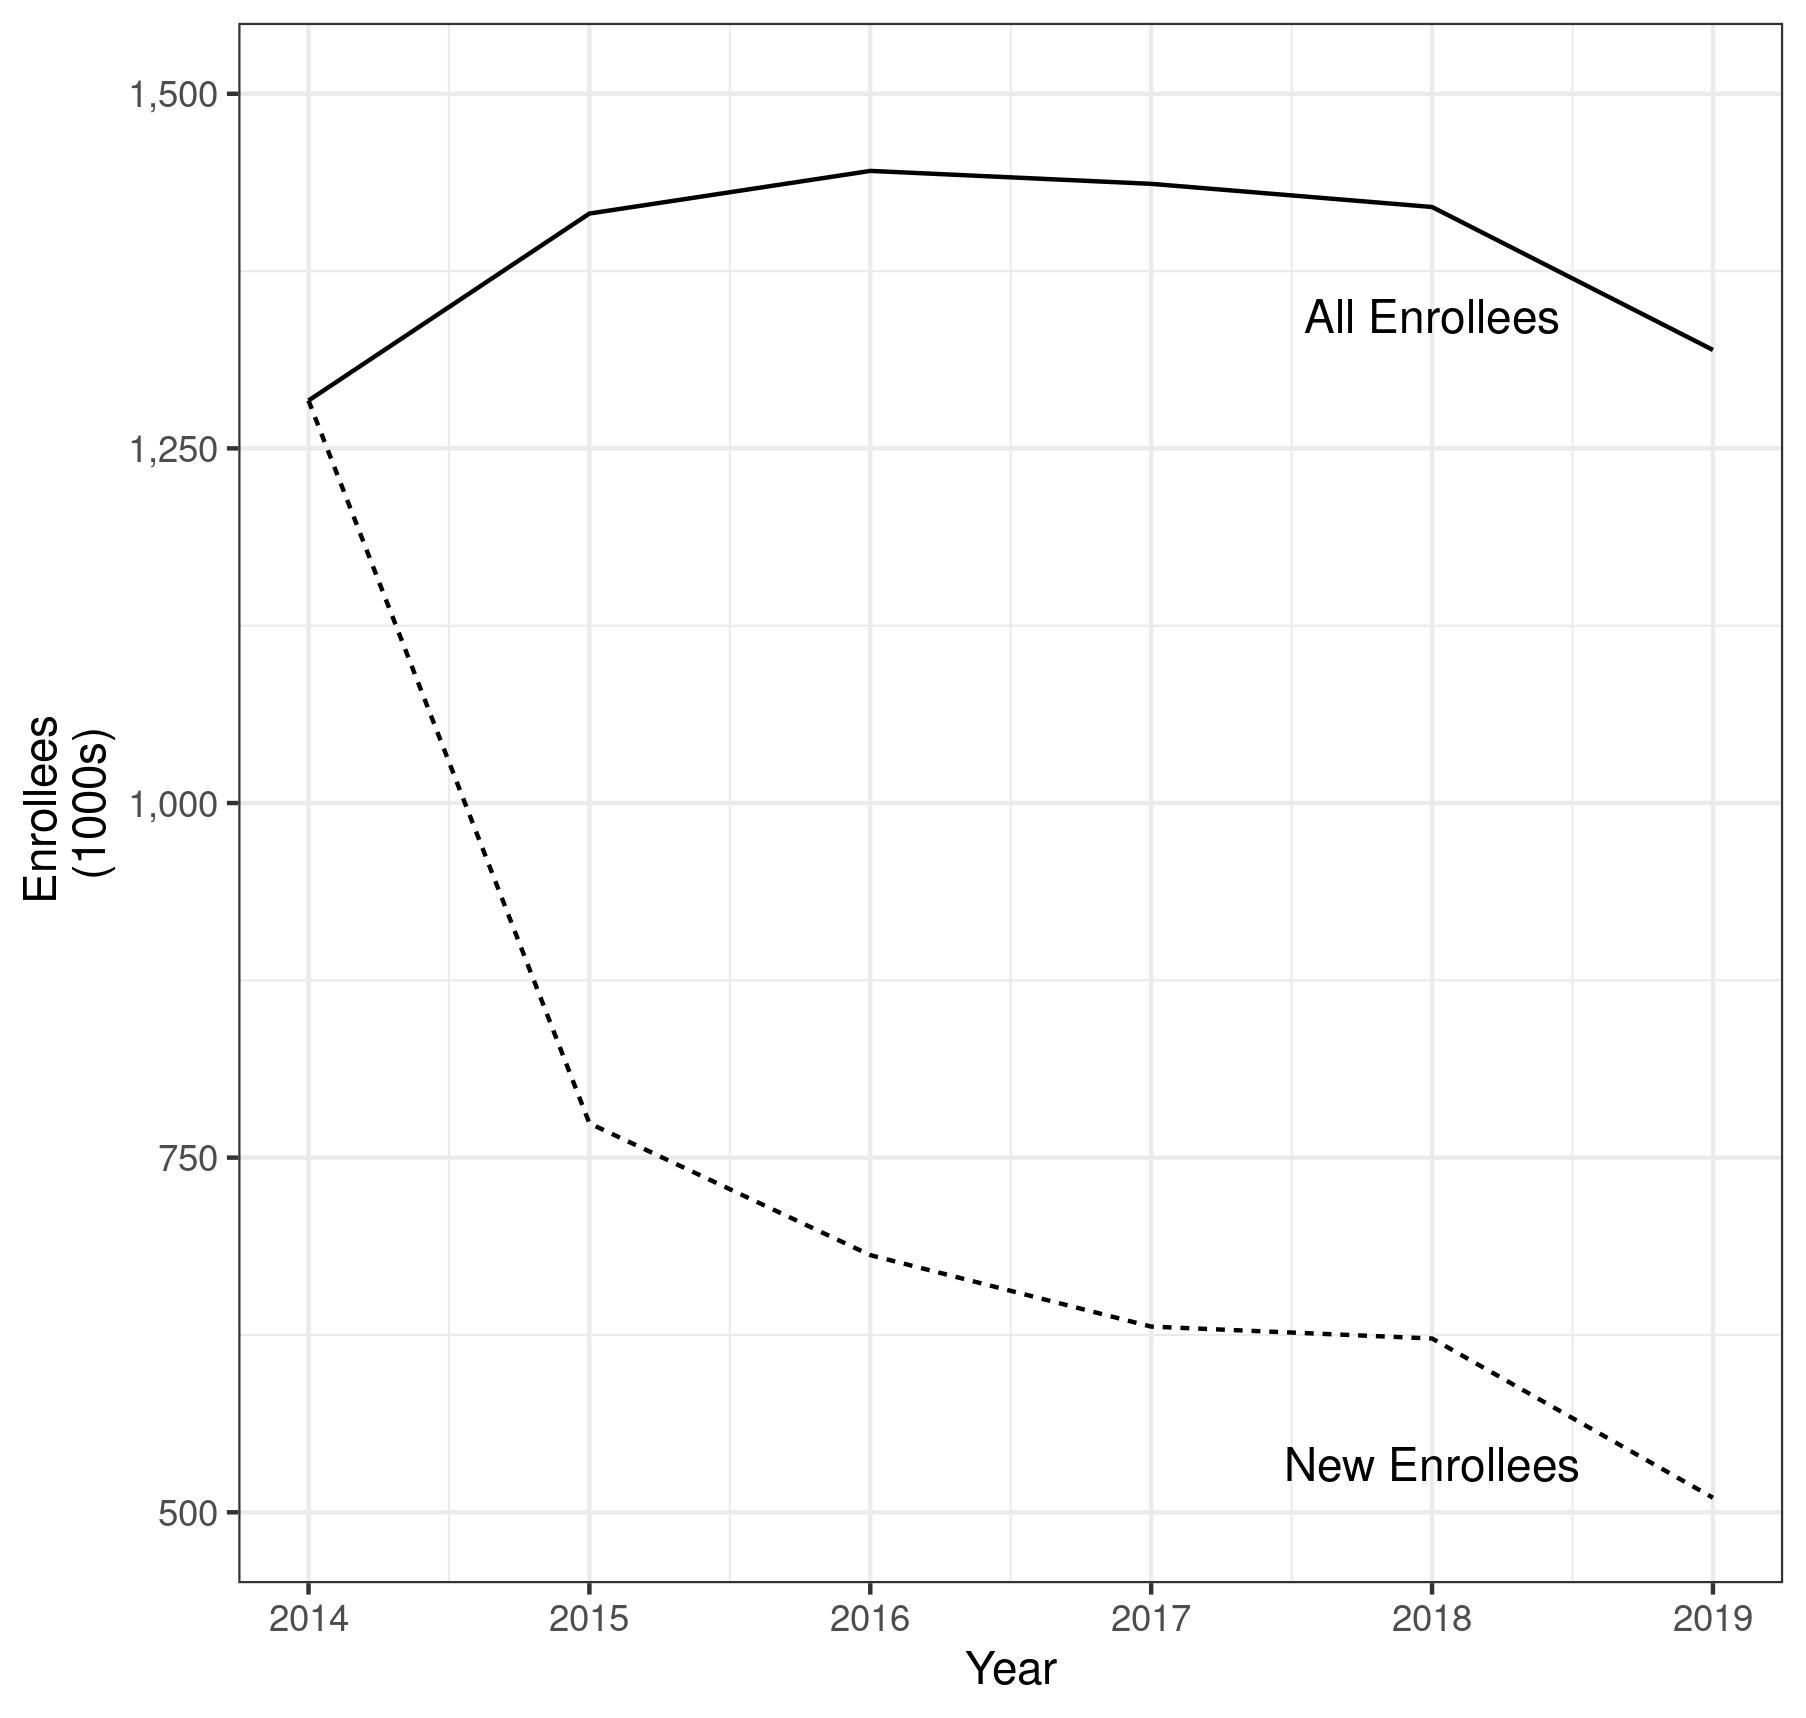
\includegraphics[scale=.7]{figures/enrollee_count.png}
 		\begin{minipage}{\textwidth}
		\bigskip
			\footnotesize \textsc{Notes:} The coefficients for high ratings are shown with circles, those for middle ratings are shown with triangles, and no reviews are shown with diamonds. The main results are designated in blue along with an indicator for specification ``Main". Various specifications and required minimum number of reviews are also indicated. 
 		\end{minipage}
 		\label{figure:SpecCurve}
 \end{figure}

\end{document}
